\chapter[Proposta Metodológica]{Proposta Metodológica}
Este capítulo apresenta os procedimentos e métodos a serem utilizados para desenvolvimento deste
 trabalho, detalhando as metodologias \textit{Bottom-Up}, utilizadas nas implementações tanto em hardware
 quanto em software, além das linguagens de programação utilizadas nas implementações e suas respectivas
 ferramentas. Por fim é apresentado um cronograma de atividades.

\section{Implementação em hardware}
Esta seção apresenta os dispositivos e ferramentas a serem utilizados neste presente trabalho, além das metodologias a serem desenvolvidas, para implementação do algoritmo de treinamento do classificador LDA em Hardware.

\subsection{Dispositivos e ferramentas}
O algoritmo de treinamento do classificador LDA será implementado nas lógicas digitais da FPGA na plataforma Zynq da placa \textit{Zybo-Board}, utilizando \textit{IP-Cores} de cálculo aritmético em ponto flutuante, que são blocos matemáticos desenvolvidos com propriedades intelectuais \cite{munoz2010tradeoff} em unidade de ponto flutuante desenvolvidos por \cite{munoz2010tradeoff} e a linguagem descrição de hardware VHDL, a fim de paralelizar os processos do algoritmo. Para o mapeamento do algoritmo em VHDL será utilizado a plataforma \textit{Vivado}, que possui todas as ferramentas necessárias para descrição, simulação, síntese e implementação para FPGAs da \textit{Xilinx} \cite{zynqBook}.

\subsection{Metodologias de desenvolvimento}
Para implementação do algoritmo de treinamento do classificador LDA em FPGA será adotada a metodologia \textit{bottom-up}, na qual cada sub-bloco desenvolvido é testado antes de ser inserido ao bloco principal, bloco de integração de todos sub-blocos do projeto, também conhecido como \textit{Top module}.
Após a implementação e simulação do \textit{Top module}, será utilizado para teste e validação do hardware
 o \textit{dataset IVa} do \textit{BCI Competition III}, além de uma análise estatística do erro apresentado
usando como modelo de referência a implementação na plataforma \textit{Matlab} por \cite{F.Lotte}.

Para validação da eficiência do SoC serão coletados os dados das seguintes características:
\begin{itemize}
	\item Consumo de hardware: LUTs, FFs, blocos de DSP, blocos de memória RAM, I/O, MUX;
	\item Dados de desempenho: frequência de operação e tempo de execução;
	\item Estimação do consumo de energético.
	\item Estimação estatístico do erro de implementação.
\end{itemize}

Os processos de implementação do hardware em um SoC é apresentado na Figura \ref{diagram_hardware}.

\begin{figure}[h]
	\centering
	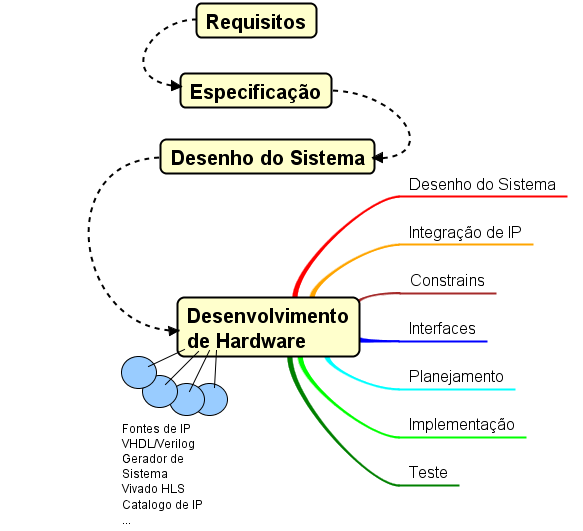
\includegraphics[keepaspectratio=true,scale=1.0]{figuras/fluxograma_hardware.PNG}
	\caption{Fluxograma de implementação de hardware em um SoC. Adaptado de \cite{zynqBook}}
	\label{diagram_hardware}
\end{figure}

\section{Implementação em software}
A seguir são apresentados os materiais, métodos e técnicas para a implementação do
algoritmo de treinamento do classificador LDA em software.

\subsection{Materiais}

Dispondo do SoC embarcado no kit de desenvolvimento da \textit{Zybo} (Digilent) , a implementação do algoritmo em 
software, explorará o processador \textit{ARM  Cortex -A9} de dois núcleos no \textit{Xilinx Zynq -7000}, usando também
o auxílio do sistema operacional \textit{Xilinux}. A codificação do algoritmo será feita na linguagem de programação \textit{C++}.

\subsection{Métodos e Técnicas}
 
Para o auxílio desta implementação, será instalado o sistema operacional \textit{Xilinux}, cujo os recursos e passos necessários
para a instalação do SO estão contidos em \cite{zynqBook}.
O processo para implementação seguirá o método \textit{bottom-up}, blocos de códigos menores serão implementados e testados
separadamente, com a finalização de todos os blocos serem integrados e testado em um único bloco principal. As entradas
para programa desenvolvido são provenientes do \textit{dataset IVa} do \textit{BCI Competition III}.

 
Os dados para análise após a implementação e teste serão:
\begin{itemize}[noitemsep]
\item Consumo de memória
\item Tempo de execução
\item Consumo de potência
\item Erro da implementação em comparação aos resultados obtidos por \cite{F.Lotte}
\end{itemize}

\section{\textit{Data Set IVa}}

Em ambas as implementações serão utilizadas o \textit{Data Set IVa} da \textit{BCI Competition III} \cite{BCICompetition}, para efeito de testes e validações do sistema.
Os dados \textit{Data Set IVa} foram adquiridos e armazenados utilizando amplificadores do tipo \textit{BrainAmp} e uma capa de eletrodos de 128 canais. Foram utilizados 118 canais de EEG posicionados de acordo com o sistema 10-20. Cada um destes canais foram filtrados em banda passante, utilizando um filtro \textit{butterworth} de quinta ordem entre as frequências de 0,05 e 200 Hz, posteriormente foram digitalizados com uma frequência de amostragem de 1 kHz com precisão de 16 bits, apresentando uma resolução de 0,1 $\mu$V, além disso também foram disponibilizados os mesmos dados com uma frequência de amostragem de 100 Hz \cite{siteBCI}.
\vspace{\onelineskip}

\section{Cronograma de Atividades}
Esta seção apresenta o cronograma de desenvolvimento deste presente trabalho.

As atividades referentes a cada um dos autores já desenvolvidas são apresentadas no cronograma da Figura \ref{cronograma}.

\begin{figure}[h]
	\centering
	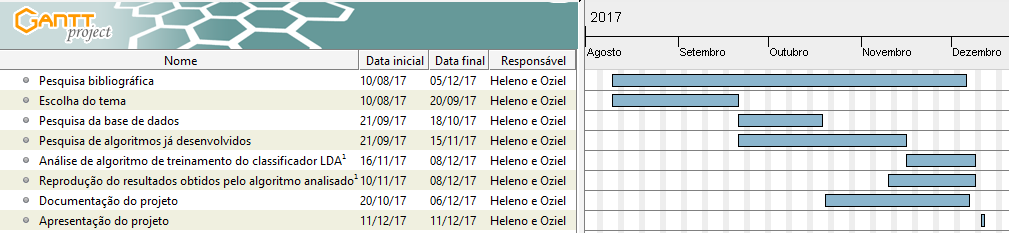
\includegraphics[keepaspectratio=true,scale=0.6]{figuras/cronograma.PNG}
	\caption{Cronograma de atividades já desenvolvidas.}
	\label{cronograma}
\end{figure}


As atividades ainda a serem realizadas neste projeto são apresentadas na Figura \ref{cronograma2}.

\begin{figure}[h]
	\centering
	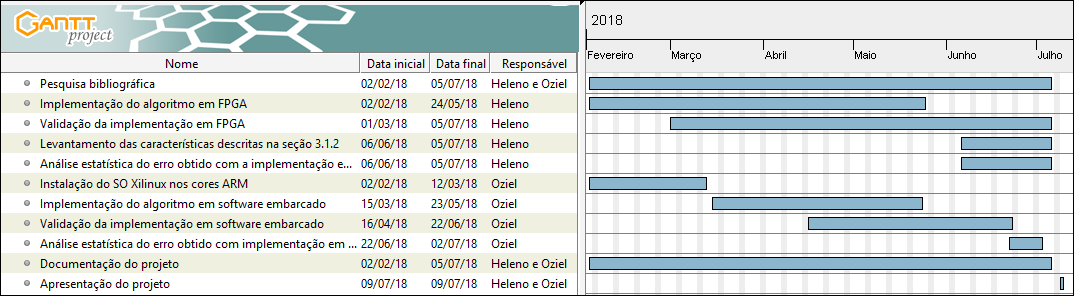
\includegraphics[keepaspectratio=true,scale=0.55]{figuras/cronograma2.PNG}
	\caption{Cronograma de atividades a serem desenvolvidas.}
	\label{cronograma2}
\end{figure}
